\section{Coupling through preCICE}
When a physical problem becomes too complex, one often split it into smaller pieces that are better manageable. These pieces, or physical fields, can then be solved separately and their solutions can be combined to an overall solution. This approach is called ``partitioned approach'' \cite{gatzhammer2015efficient}. This approach allows to reuse the simulation code for the single fields and simultaneously provides the possibility to encapsulate the coupling functionality itself as a reusable component, too. This allows minimal access to solver codes, i.e., treating them as black boxes. At the same time the solver code does not have to include the whole coupling code making it less application dependent. The coupling tool preCICE offers coupling functionality to develop a multi-physics simulation environment using existing solvers. In this work a fluid-structure interaction (FSI) will be simulated. The thesis' program represents the structure part whereas the fluid part can be dynamically exchanged due to the coupling with preCICE. This Chapter gives an overview of preCICE and its main components and shows the implementation modifications that were necessary to integrate preCICE and prepare the code for coupling.

 \subsection{Overview of preCICE} %gelbe Marker
  The goal of preCICE is to provide all functionality to realize a multi-physics simulation environment working with existing single-physics solvers. This includes simulations like fluid-structure, fluid-acoustics, fluid-solid thermodynamics and porous-free flow interactions, for instance. It provides technical inter-code communication via MPI or TCP/IP, methods for data mapping between different grids and coupling methods based on quasi-Newton methods to ease the development process. preCICE supports parallel solvers through efficient point-to-point communication without the need of a server instance. It also features a high-level API making its integration into existing solver code minimal invasive \cite{bungartz2015fully}.
  
  preCICE supports partitioned coupling of black box solvers with focus on FSI and provides a geometry interface for Cartesian grid solvers. Its API is available for C++, C, and Fortran and consists of high-level methods enabling solvers to use coupling functionality in a flexible way. After the preCICE integration into the solver's code, a peer-to-peer communication without central control instance is generated. The single solver codes can be run serial or parallel without major modifications to the integrated API. Furthermore, the concrete coupling algorithms in the simulation can be selected through an XML configuration file that optimizes the solver adaption \cite{gatzhammer2015efficient}.
  
  \begin{figure}[htbp]
  	\centering
  	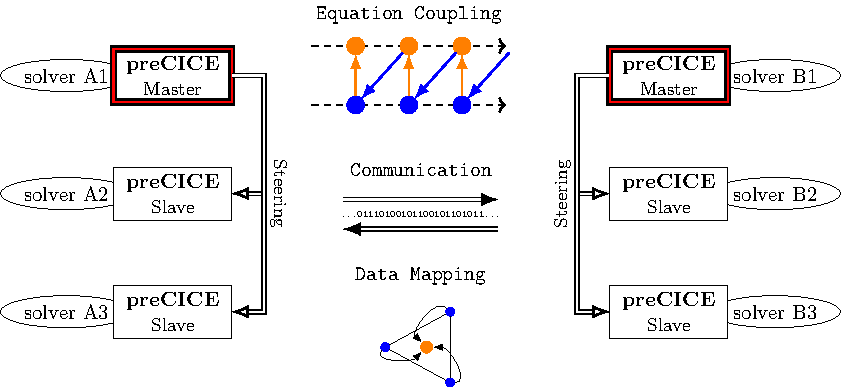
\includegraphics[width=0.97\linewidth]{figures/NewCommunicationScheme}
  	\caption{Schematic view of a partitioned multi-physics simulation with two solvers (A and B) coupled through preCICE. In the middle are the three main functionalities of preCICE shown, that steer coupling iterations: Fix-point acceleration methods, point-to-point communication and data mapping between non-matching grids at the coupling interface. Picture courtesy of Florian Lindner \cite{bungartz2015fully} }
  	\label{fig:precice}
  \end{figure}
  
  Figure \ref{fig:precice} shows a schematic view of the main functionality groups of preCICE. Two solvers (A and B) are coupled through the preCICE tool. The three main functionalities of preCICE are drawn in the middle: Fix-point acceleration methods, point-to-point solver process communication and data mapping between non-matching grids at the coupling surface. Each shown solver runs in parallel with a master process controlling tasks such as convergence for the corresponding solver as well as for the whole simulation. The following sections describe each of the three addressed main functionalities in greater detail.
  
 
 \subsection{Coupling Methods} % türkise Marker
  preCICE distinguishes two possible coupling schemes: Explicit and implicit coupling. A single time step of multi-physics simulation partitioned into several solvers can be done with only a small and fixed number of calls of time steps per solver. This is described by an explicit coupling scheme. The alternative is an iterative procedure that achieves convergence with respect to the monolithic solution of the system in each time step. An implicit coupling scheme then iterates over a coupling equation until convergence occurs. Based on \cite{bungartz2015fully} it is assumed that two solvers $S_1$ and $S_2$ make up a coupled system. Vector spaces $X_1$ and $X_2$ describe data at the coupling interface to be mapped between the two solvers in a single time step. The output of $S_1$ is required as an input by $S_2$ and vice versa, i.e. it follows:
  \begin{equation}
  S_1: X_1 \leftarrow X_2\quad \text{and}\quad S_2:X_2 \leftarrow X_1
  \end{equation}
  The fluid-structure coupling done in this work, is an example for a Dirichlet-Neumann type coupling. The displacements at the coupling interface of the structure solver is the input for the fluid solver that gives forces to the structure solver as its output.
 
  \subsubsection{Explicit Coupling Schemes}
   Two different implementations of explicit coupling schemes exist in preCICE: The staggered scheme and the parallel scheme. The staggered scheme uses the old time step's values $x_1^{(n)}$ at the coupling surface for the execution of the $n$th time step ($t_n \leftarrow t_{n+1}$) to achieve $x_2^{(n+1)}$. These new values act as boundary values for the $n$th time step of $S_2$ \cite{bungartz2015fully}:
   \begin{equation}
   x_2^{(n+1)} = S_1^{(n)}\left( x_1^{(n)} \right)\quad \text{and}\quad x_1^{(n+1)} = S_2^{(n)}\left( x_2^{(n+1)} \right)
   \end{equation}
   Since the two solvers are executed staggered, this scheme is not optimal with respect to load balancing \cite{bungartz2015fully}. In contrast, the parallel scheme does not have this drawback. It uses the old time step values $x_1^{(n)}$ and $x_2^{(n)}$ as inputs for both solvers:
   \begin{equation}
   x_2^{(n+1)} = S_1^{(n)}\left( x_1^{(n)} \right)\quad \text{and}\quad x_1^{(n+1)} = S_2^{(n)}\left( x_2^{(n)} \right)
   \end{equation}
   According to \cite{bungartz2015fully} both explicit schemes yield consistent time steps but cause instabilities that cannot be avoided, even if the time step length is reduced.
  
  \subsubsection{Implicit Coupling Schemes}
   All implicit coupling schemes in preCICE are based on fixed-point iterations using the staggered or the parallel explicit scheme. The fixed-point iteration regarding the staggered scheme is as follows:
   \begin{equation}
   x_2^{(n+1),i+1} = S_1^{(n)}\left( x_1^{(n+1),i} \right)\quad \text{and}\quad x_1^{(n+1),i+1} = S_2^{(n)}\left( x_2^{(n+1),i+1} \right)
   \end{equation}
   The fixed-point iteration corresponding to the parallel scheme can be written as:
   \begin{equation}
   x_2^{(n+1),i+1} = S_1^{(n)}\left( x_1^{(n+1),i} \right)\quad \text{and}\quad x_1^{(n+1),i+1} = S_2^{(n)}\left( x_2^{(n+1),i} \right)
   \end{equation}
   Here, the new iterates for $x_2^{(n+1),i+1}$ and $x_2^{(n+1),i+1}$ are computed in parallel. preCICE offers simple underrelaxation, adaptive Aitken underrelaxation and various quasi-Newton solvers in order to solve these fixed-point equations in as robust and stable as possible \cite{bungartz2015fully}. In the following a generic fixed-point equation
   \begin{equation}\label{eq:fixed-point-eq}
   x = H(x)
   \end{equation}
   is considered. Every fixed-point equation solver in preCICE is a combination of a fixed-point iteration and a post-processing step that modifies the result of the fixed-point iterator. Underrelaxed fixed-point iterations are the simplest solvers \cite{bungartz2015fully}:
   \begin{equation}
   x^{i+1} = H(x^i)+(\omega - 1)\left( H(x^i) - x^i\right)
   \end{equation}
   with $\omega \in \mathbb{R}, 0 < \omega \leq 1$ either a user-defined value or additionally adapted by the solver throughout the iterations using Aitken underrelaxation.
   In order to get the full potential of a parallel scheme, preCICE provides a powerful class of convergence acceleration methods, called quasi-Newton methods. With these methods a fast convergence is achieved in particular for difficult problems when using parallel fixed-point iterations \cite{bungartz2015fully}. All quasi-Newton methods in preCICE accelerate the fixed-point iteration by a subsequent Newton step \cite{bungartz2015fully}:
   \begin{align}
   x^{k+1} = \underbrace{H(x^k)} - J_{\tilde{R}}^{-1}\left( \underbrace{H(x^k) - x^k}\right) \\
   =: \tilde{x}^k\qquad =\tilde{x}^k - H^{-1}(\tilde{x}^k) \nonumber
   \end{align}
   where $\tilde{R} = I-H^{-1}$ maps $\tilde{x}^k$ to the residual $r^k=\tilde{R}(\tilde{x}^k)=H(x^k)-x^k$. The inverse of the Jacobian $J_{\tilde{R}}^{-1}$ can be approximated ($\hat{J}_{\tilde{R},k}^{-1}$) in different ways in preCICE:
   \begin{itemize}
   	\item The classical interface quasi-Newton (IQN) approach uses the approximated inverse Jacobian with minimal Frobenius norm:
   	\begin{equation}
   	\left\| \hat{J}_{\tilde{R},k}^{-1} \right\|_F \leftarrow \min
   	\end{equation}
   	\item The multi-vector quasi-Newton (IMVJ) approach minimizes the distance between $\hat{J}_{\tilde{R},k}^{-1}$ and the approximate $\hat{J}_{\tilde{R},k}^{-1,(n)}$ from the last time step:
   	\begin{equation}
   	\left\| \hat{J}_{\tilde{R},k}^{-1} - \hat{J}_{\tilde{R},k}^{-1,(n)}\right\|_F \leftarrow \min
   	\end{equation}
   \end{itemize}
   For more details, see \cite{bungartz2015fully} and \cite{gatzhammer2015efficient}.
   
   Additional specifications can be made by the user to adapt the coupling method to the problem. A statement of extrapolation in time can be made to get a better initial guess for the next time step solution and with subcycling several small time steps are done in one of the solvers while the others use a larger time step.
  

 \subsection{Data Mapping} % rosa Marker
  Due to the fact that independent solvers are used for coupling, it can happen that the single solver meshes are non-matching. This requires a mapping of the data that is sent by the above iterative coupling methods from the coupling surface of one solver domain to the surface of the other solver domain. The case where the two meshes matching each other is not very common when dealing with two distinct solvers and would only result in a copying of data values for transfer without any interpolation or projection. In the case of non-conforming meshes interpolation algorithms are necessary and when the two grids overlap or gaps exist even projections in some form are additionally required \cite{gatzhammer2015efficient}. preCICE offers some data mapping methods but also provides the possibility for user-defined mapping implementations for special needs \cite{bungartz2015fully}.
  \subsubsection{Conservative vs.\ Consistent}
   The mapping of displacements and pressures, for example, usually requires a \textbf{consistent mapping}, i.e. constants should be interpolated exactly. Let $\underline{H}_{AB} \in \mathbb{R}^{n_A \times n_B}$ be the matrix mapping values between variables from solver $A$ to $B$. Then consistent mapping can be expressed as follows:
   \begin{equation}
   \underline{\beta}_B = \underline{H}_{AB} \underline{\beta}_A
   \end{equation}
   with the arbitrary variable $\beta$ whose values are represented as matrix $\beta_{A,i} = \beta_{B,j} = \beta = const, 1 \leq i \leq n_A, 1 \leq j \leq n_B$. The property of exact constant interpolation is the case if and only if the row sums of the mapping matrix are equal to 1 \cite{gatzhammer2015efficient}:
   \begin{equation}
   \beta_{B,i} = \sum_{j=1}^{n_A} H_{AB,ij}\beta_{A,j} = \beta_{A,j} = \beta \qquad \forall i
   \end{equation}
   
   A \textbf{conservative mapping} on the other hand is important for integral values like forces. This mapping approach requires the sum of the data values is equal on both sides:
   \begin{equation}
   \sum_{i=1}^{n_B}\beta_{B,i} = \sum_{j=1}^{n_A}\beta_{A,j}
   \end{equation}
   This property holds only for the column sums of $\underline{H}_{AB}$ to be equal to 1:
   \begin{equation}
   \sum_{i=1}^{n_B}\beta_{B,i} = \sum_{i=1}^{n_B}\left( \underline{H}_{AB}\underline{\beta}_A \right)_i = \sum_{i=1}^{n_B}\sum_{j=1}^{n_A} H_{AB,ij}\beta_{A,j} = \sum_{j=1}^{n_A}\left( \sum_{i=1}^{n_B} H_{AB,ij}\right) \beta_{A,j} = \sum_{j=1}^{n_A} 1 \beta_{A,j}
   \end{equation}
   Further details to the mathematical background of the two mapping approaches can be found in \cite{gatzhammer2015efficient}. Both mappings are available for all methods described below.

  \subsubsection{Nearest-Neighbor}
   The Nearest-Neighbor mapping method works locally and requires only vertex positions, i.e. only the data nodes of the solver surface meshes are required for the mapping. The mapping itself is simple: In order to map values from mesh A to mesh B, for every node of mesh B the geometrically closet neighbor to a node of mesh A needs to be determined. Then, the data value from the closest node in mesh A is copied to the corresponding node in mesh B. There are special cases that can happen with this projection method: A value from mesh A can be copied to more than one node of mesh B if the node in mesh A is closest to all of the B nodes. On the other hand, nodes in A can be omitted if no projection partner in B were found, since the search for nearest neighbors is done on mesh B only. This is a general problem of all projection methods \cite{gatzhammer2015efficient}.
   
   If the meshes have matching vertex positions then this mapping method is good choice. For non-conforming meshes the first order accuracy of Nearest-Neighbor makes it a rather bad choice and other mapping methods should be taken into account \cite{bungartz2015fully}.
  
  \subsubsection{Nearest-Projection}
   The Nearest-Projection mapping requires not only vertex positions but also topology information for the source mesh. It searches for mesh nodes on the target mesh and creates geometrical projections to a matching set of elements on the source mesh. An interpolation is employed from nodes to mesh elements and vice versa. The finding of closest neighbors is similar to Nearest-Neighbor, but Nearest-Projection uses faces instead of points for its projections and several data nodes can be involved \cite{gatzhammer2015efficient}. Just as for the Nearest-Neighbor mapping, nodes can be omitted here if the mesh widths differ too much locally and theoretically this method is also of first order due to the projection. In practice, due to the fact that often the distance between the two meshes normal to the coupling interface is smaller that the mesh widths, a second order accuracy can be observed \cite{bungartz2015fully}.
  
  \subsubsection{Radial Basis Function}
   This mapping method uses radial basis functions (RBF) centered at the mesh nodes of the source mesh. It does not require topological information, projections or search-algorithms. It works well on general non-conforming meshes, where overlapping meshes or gaps between them can occur. Several different basis functions are implemented in preCICE, including Gaussian, (Inverse) Multiquadrics, Thin Plate Splines, Volume Splines (see \cite{bungartz2015fully}), but further functions can be added easily. The global support of some RBFs (Gaussian and Thin Plate, for instance) can be limited to a smaller area by introducing a cut-off radius. This reduces the density of the system matrix for interpolation and thus reduces the amount of communication between the solvers and the computational complexity of the data mapping. This allows local communication while still having the properties of the radial basis functions \cite{bungartz2015fully}.


 \subsection{Communication} % hellblaue Marker
  The coupling of different solvers in the frame of a multi-physics simulation requires an efficient communication between different executables. preCICE offers a communication per interaction of two or more participants. Either MPI ports or low level TCP/IP sockets are available for communication in preCICE. A fully parallel point-to-point data transfer is possible with preCICE, since it analyses the mesh decomposition of all participants and constructs only local communication channels where they are needed \cite{bungartz2015fully}.
 
  \subsubsection{MPI Communication}
   The message passing interface (MPI) is used in preCICE with a multiple program multiple data paradigm, i.e. two different codes are communicating with their own data. Two MPI-based communication methods are implemented which differ in the way how they set up the communication space. With the first method all executables are put in the same communication space, called ``communicator world''. All processes of each participant are then grouped into separate communicators. An inter-communicator is used as the actual channel for data exchange.
   The second method establishes a connection between processes started individually and in different communication spaces. The exchange of connection information is done through a commonly accessible file which stores the port names of the participants. For this a MPI version of 2 or greater is needed \cite{gatzhammer2015efficient}. The result is the same as with method one: An inter-communicator.
   
  \subsubsection{Socket Communication}
   The communication by TCP/IP increases compatibility to closed-source software that might be restricted to some MPI implementations \cite{bungartz2015fully}. To abstract from platform dependent socket interfaces like Pthreads or Winsock, the Boost.Asio (asynchronous network and low-level input/output) library was used for implementing the socket communication in preCICE \cite{gatzhammer2015efficient}. The sending and receiving of data is managed by the transfer control protocol (TCP) which is designed for failsafe data transfer and synchronization between sender and receiver. Communication via TCP is not typical for multi-physics simulations that often run on supercomputers, because it involves a synchronization step and additional communication overhead compared to MPI. Other difficulties are that ports used for socket communication may be blocked by default and each supercomputer node might have different network address which requires automated checks on a low-level socket layer \cite{gatzhammer2015efficient}.


 \subsection{Implementation}
 % TODO: text
 
  \subsubsection{Additional Boundary Conditions}
   \begin{itemize}
  	\item - 2: inner node, part of preCICE interface region (only used by preCICE coupled variant)\\
  	- 20: same as 0 but additionally part of preCICE interface region (only used...)\\
  	- 21: same as 1 but additionally part of preCICE ...
  	\end{itemize}
  
  	
  \subsubsection{Partitioned Coupling Surface}
   the surface interface between the solvers is partitioned across the mpi processes of the structure solver. every process needs to construct a grid for itself
   
   
  \subsubsection{Integration of preCICE}
   the main-function gets modified with the preCICE code
 
\newpage